\section{Introducere}
\begin{frame}[c,allowframebreaks]{Introducere}
Importan\c{t}a ciocnirilor la energii joase\\
\begin{itemize}
  \item studiul r\u{a}cirii gazelor prin evaporare \^{i}n capcane magnetice
  \item manipularea optic\u{a} a proceselor de r\u{a}cire (cu laseri)
  \item m\u{a}surarea cu precizie a parametrilor atomici \c{s}i moleculari
  \item studiul coeren\c{t}elor materie-und\u{a} ce apar la energii joase
  \item statistica condensa\c{t}ilor cuantici forma\c{t}i din atomi ce interac\c{t}ioneaz\u{a} slab
\end{itemize}

Scopul lucr\u{a}rii:
C\u{a}utam s\u{a} demonstr\u{a}m c\u{a} ciocnirile la energii joase pot fi descrise printr-un unic parametru: lungimea de \^{i}mpr\u{a}\c{s}tiere. Ne propunem s\u{a} calcul\u{a}m acest parametru pentru c\^{a}teva poten\c{t}iale simple, apoi vom  aplica algoritmul \c{s}i pentru un poten\c{t}ial de interac\c{t}ie aproximat penru ciocnirile atomilor de Cesiu. 

\end{frame}

\section{Elemente de teoria ciocnirilor}

\subsection{Ciocniri \^{i}n mecanica clasic\u{a}}
\begin{frame}[allowframebreaks]{Ciocniri \^{i}n mecanica clasic\u{a}}
\^{I}ntr-un experiment de \^{i}mpr\u{a}\c{s}tiere, se observ\u{a} ciocniri \^{i}ntre un fascicul de particule incidente \c{s}i un material \c{t}int\u{a}.\\

Num\u{a}rul de particule \^{i}mpr\u{a}\c{s}tiate $dN$ \^{i}ntr-un element de unghi solid $d\Omega$  este propor\c{t}ional cu o cantiate care joac\u{a} un rol central \^{i}n fizica \^{i}mpr\u{a}\c{s}tierilor: sec\c{t}iunea diferen\c{t}ial\u{a} de \^{i}mpr\u{a}\c{s}tiere:
\begin{align}
\frac{d\sigma(\theta,\varphi)}{d\Omega}=\frac{1}{J_{inc}}\frac{dN(\theta,\varphi)}{d\Omega}
\end{align}

unde $J_{inc}$ este fluxul incident de particule \c{s}i $\sigma$ reprezint\u{a} sec\c{t}iunea total\u{a} de \^{i}mpr\u{a}\c{s}tiere.
\begin{align}
\sigma=\int\frac{d\sigma}{d\Omega}d\Omega=\int_{0}^{\pi}\sin\theta d\theta\int_{0}^{2\pi}\frac{d\sigma(\theta,\varphi)}{d\Omega}d\varphi
\end{align} 
\end{frame}


\begin{frame}[allowframebreaks]{SL \c{s}i SCM}
Este important s\u{a} distingem cele dou\u{a} sisteme de referin\c{t}\u{a} la care ne raport\u{a}m c\^{a}nd efectu\u{a}m un experiment de \^impr\u{a}\c{s}tiere: sistemul laboratorului (SL) \c{s}i sistemul centrului de mas\u{a} (SCM).
\begin{align}
\left(\frac{d\sigma}{d\Omega_1}\right)_{SL}=\frac{(1+\frac{m^2_1}{m^2_2}+2\frac{m_1}{m_2}\cos\theta)^{3/2}}{1+\frac{m_1}{m_2}\cos\theta}\left(\frac{d\sigma}{d\Omega}\right)_{SCM}
\end{align}
\\
Cazuri limit\u{a}:\\
a) $m_2\gg m_1$ sau $\frac{m_1}{m_2} \xrightarrow{}0$ rezultatele in SL \c{s}i SCM sunt identice $\left(\frac{d\sigma}{d\Omega_1}\right)_{SL}=\left(\frac{d\sigma}{d\Omega}\right)_{SCM}$ deoarece $\theta_1=\theta$\\
b) $m_2=m_1$ atunci $\tan\theta_1=\tan\frac{\theta}{2}$ sau $\theta_1=\frac{\theta}{2}$ rezult\^{a}nd 
\begin{align}
\boxed{\left(\frac{d\sigma}{d\Omega_1}\right)_{SL}=4\left(\frac{d\sigma}{d\Omega}\right)_{SCM}\cos\frac{\theta}{2}}
\end{align}


\end{frame} 

\subsection{Ecua\c{t}ia Schr\"{o}dinger.}
\begin{frame}[allowframebreaks]{Ecuatia Schr\"{o}dinger}
Consider\u{a}m \^impr\u{a}\c{s}tierea a dou\u{a} particule non-relativiste, far\u{a} spin, de mase $m_1,m_2$ sau analog, \^impr\u{a}\c{s}tierea unei particule de mas\u{a} redus\u{a} $\mu$ pe un poten\c{t}ial central.
Problema \^{i}mpr\u{a}\c{s}tierii a dou\u{a} particule se reduce la rezolvarea ecua\c{t}iei Schr\"{o}dinger:
\begin{align}
-\frac{\hbar^2}{2\mu}\nabla^2\psi({\bm r})+V({\bm r})\psi({\bm r})=E\psi({\bm r})
\end{align}
Presupun\^{a}nd c\u{a} poten\c{t}ialul are raza de ac\c{t}iune finit\u{a} \c{s}i c\u{a} func\c{t}ia de und\u{a} ce descrie \^{i}mpr\u{a}\c{s}tierea este o superpozi\c{t}ie a undei plane incidente \c{s}i a undei sferice \^{i}mpr\u{a}\c{s}tiate putem scrie:
\begin{align}
&\psi({\bm r})=\phi_{inc}({\bm r})+\phi_{sc}({\bm r})\\
&\phi_{inc}({\bm r})=Ae^{i{\bm k_0}\cdot{\bm r}} \qquad \phi_{sc}({\bm r})=A f(\theta,\varphi)\frac{e^{i{\bm k}\cdot{\bm r}}}{r}\\
&\psi({\bm r})=A \left[ e^{i{\bm k_0}\cdot{\bm r}}+f(\theta,\varphi)\frac{e^{i{\bm k}\cdot{\bm r}}}{r}\right]
\end{align}
{\bf unde $f(\theta,\varphi)$ reprezint\u{a} amplitudinea de \^{i}mpr\u{a}\c{s}tiere.}
\end{frame} 


\begin{frame}[allowframebreaks]{Amplitudinea de \^{i}mpr\u{a}\c{s}tiere}
C\u{a}ut\u{a}m conexiunea dintre amplitudinea de \^{i}mpr\u{a}\c{s}tiere \c{s}i sec\c{t}iunea diferen\c{t}ial\u{a} de \^{i}mpr\u{a}\c{s}tiere.
Introducem densit\u{a}\c{t}ile de flux: 
\begin{align}
&J_{inc}=|A|^2 \frac{\hbar k_0}{\mu}\\
&J_{sc}=|A|^2 \frac{\hbar k}{\mu r^2}|f(\theta,\varphi)|^2=\frac{k}{k_0}\frac{J_{inc}}{r^2}|f(\theta,\varphi)|^2
\end{align}
Num\u{a}rul de particule \^{i}mpr\u{a}\c{s}tiate:
\begin{align}
dN(\theta,\varphi)=J_{sc}r^2d\Omega
\end{align}
Folosind aceast rezultat \c{s}i defini\c{t}ia sec\c{t}iunii diferen\c{t}iale ob\c{t}inem:
\begin{align}
\frac{d\sigma}{d\Omega}=\frac{1}{J_{inc}}\frac{dN}{d\Omega}=\frac{1}{J_{inc}}J_{sc}r^2=\frac{k}{k_0}|f(\theta,\varphi)|^2
\end{align}
\^{I}n cazul \^{i}mpr\u{a}\c{s}tierilor elastice $k=k_0$, deci ob\c{t}inem:
\begin{align}
\frac{d\sigma}{d\Omega}=|f(\theta,\varphi)|^2
\end{align}

\newpage

\^{I}n cele ce urmeaz\u{a} ar\u{a}t\u{a}m c\u{a} amplitudinea de \^{i}mpr\u{a}\c{s}tiere poate fi ob\c{t}inut\u{a} dintr-o form\u{a} asimptotic\u{a} a solu\c{t}iei ecua\c{t}iei Schr\"{o}dinger.
\begin{align}
(\nabla^2+k^2)\psi({\bm r})=\frac{2\mu}{\hbar^2}V({\bm r})\psi({\bm r}) 
\end{align}
Solu\c{t}ia general\u{a} a acestei ecua\c{t}ii este o sum\u{a} de dou\u{a} componente: o solu\c{t}ie general\u{a} a ecua\c{t}iei omogene:
\begin{align}
(\nabla^2+k^2)\psi_{omog}({\bm r})=0
\end{align}
\c{s}i o solu\c{t}ie particular\u{a} pe care o exprim\u{a}m cu ajutorul func\c{t}iei Green. Deci solu\c{t}ia general\u{a} este:
\begin{align}
\psi({\bm r})=\phi_{inc}({\bm r})+\frac{2\mu}{\hbar^2}\int G({\bm r}-{\bm r'})V({\bm r'})\psi({\bm r'})d^3r' \label{ecuatie236}
\end{align} 
\begin{align}
\psi({\bm r})=\phi_{inc}({\bm r})-\frac{\mu}{2\pi\hbar^2}\int\frac{e^{ik|{\bm r}-{\bm r'}|}}{|{\bm r}-{\bm r'}|}V({\bm r'})\psi({\bm r'})d^3r' \label{ecuatie247}
\end{align}
\newpage

Dac\u{a} poten\c{t}ialul este destul de slab, el va distorsiona foarte pu\c{t}in unda incident\u{a}. {\bf Aproxima\c{t}ia Born} const\u{a} \^{i}n aproximarea undei \^{i}mpr\u{a}\c{s}tiate cu o und\u{a} plan\u{a}. Deci \^{i}n solu\c{t}ia general\u{a} \^{i}nlocuim pe $\psi({\bm r})$ din integrand cu $\phi({\bm r})$
\begin{align}
\psi({\bm r})=\phi_{inc}({\bm r})-\frac{\mu}{2\pi\hbar^2}\int\frac{e^{ik|{\bm r}-{\bm r'}|}}{{\bm r}-{\bm r'}}V({\bm r'})\phi_{inc}({\bm r'})d^3r'
\end{align}
Privind comportarea asimptotic\u{a}
\begin{align}
\psi({\bm r})\to e^{i{\bm k_0}\cdot{\bm r}}+\frac{e^{ikr}}{r}f(\theta,\varphi),(r\to\infty)
\end{align} 
Rezult\u{a} amplitudinea de \^{i}mpr\u{a}\c{s}tiere
\begin{align}
&f(\theta,\varphi)=-\frac{\mu}{2\pi\hbar^2}\int e^{-i{\bm k}\cdot{\bm r'}}V({\bm r'})d^3r'=-\frac{\mu}{2\pi\hbar^2}\int e^{i{\bm q}\cdot{\bm r'}}V({\bm r'})d^3r'\\
&f(\theta)=-\frac{2\mu}{\hbar^2q}\int_{0}^{\infty}r'V(r')\sin(qr')dr' ,\qquad q=2k\sin\frac{\theta}{2}\\
&\frac{d\sigma}{d\Omega}=|f(\theta)|^2=\frac{4\mu^2}{\hbar^4q^2}\left\lvert\int_{0}^{\pi}r'V(r')\sin(qr')dr'\right\rvert^2
\end{align}

\end{frame} 

\subsection{Sec\c{t}iunea de \^{i}mpr\u{a}\c{s}tiere. Limita de energii joase}
\begin{frame}[allowframebreaks]{Analiza par\c{t}ial\u{a} a undei. Defazaje}
Presupunem c\u{a} poten\c{t}ialul are simetrie sferic\u{a}. Momentul cinetic al particulei se conserv\u{a} dup\u{a} ciocnire. Presupun\^{a}nd unda incident\u{a} \^{i}n direc\c{t}ia $z$ \c{s}i $\phi_{inc}({\bm r})=exp(ikr\cos\theta)$, o putem exprima  ca o superpozi\c{t}ie de st\u{a}ri proprii ale momentului cinetic, fiecare definit\u{a} de un num\u{a}r cuantic $l$:
\begin{align}
e^{i{\bm k}\cdot{\bm r}}=e^{ikr\cos\theta}=\sum_{l=0}^{\infty}i^l(2l+1)j_l(kr)P_l(\cos\theta) 
\end{align}
unde $j_l$ sunt func\c{t}iile Bessel sferice. Reamintim:
\begin{align}
\psi({\bm r})=A \left[ e^{i{\bm k_0}\cdot{\bm r}}+f(\theta,\varphi)\frac{e^{i{\bm k}\cdot{\bm r}}}{r}\right]
\end{align}
Din cele dou\u{a} rezult\u{a}:
\begin{align}
\psi(r,\theta)\simeq\sum_{l=0}^{\infty}i^l(2l+1)j_l(kr)P_l(\cos\theta)+f(\theta)\frac{e^{ikr}}{r}
\end{align}
De asemenea, solu\c{t}ia general\u{a} a ecua\c{t}iei Schr\"{o}dinger pentru poten\c{t}ial cu simetrie sferic\u{a}:
\begin{align}
\psi(r,\theta)=\sum_{l=0}^{\infty}a_lR_{kl}(r)P_l(\cos\theta) 
\end{align}
\end{frame} 

\begin{frame}[allowframebreaks]{Forma asimptotic\u{a}}
Analiz\u{a}m forma asimptotic\u{a} a celor dou\u{a} rezultate. Ne intereseaz\u{a} \^{i}n mod deosebit forma asimptotic\u{a} a func\c{t}iei radiale $R_{kl}$ descris\u{a} cu ajutorul func\c{t}iilor Bessel
\begin{align}
&R_{kl}(r)=A_lj_l(kr)+B_ln_l(kr)\\
&R_{kl}(r) \to A_l \frac{\sin(kr-l\pi/2)}{kr}-B_l\frac{\cos(kr-l\pi/2)}{kr}
\end{align}
Renun\c{t}\u{a}m la cosinus pentru a satisface condi\c{t}iile \^{i}n origine
\begin{align}
R_{kl}(r)\to C_l\frac{sin(kr-l\pi/2+\delta_l)}{kr}
\end{align}
unde $A_l=C_l\cos\delta_l$ \c{s}i $B_l=-C_l\sin\delta_l$, deci $C_l=\sqrt{A^2_l+B^2_l}$ \c{s}i
\begin{align}
tan\delta_l=-\frac{B_l}{A_l} \Rightarrow \delta_l=-\tan^{-1}\left(\frac{B_l}{A_l}\right)
\end{align}
\end{frame} 

\begin{frame}[allowframebreaks]{Defazajul. Conexiunea cu sec\c{t}iunea diferen\c{t}ial\u{a}}

{\bf Observ\u{a}m c\u{a} dac\u{a} $\delta_l=0$, func\c{t}ia radial\u{a} $R_{kl}(r)$ este finit\u{a} \^{i}n $r=0$, deci forma asimptotic\u{a} se reduce doar la $j_l(kr)$. Deci $\delta_l$ este un unghi real care dispare pentru orice valoare a lui $l$ \^{i}n absen\c{t}a poten\c{t}ialului $(V=0)$ \c{s}i se nume\c{s}te defazaj. Acesta m\u{a}soar\u{a}, la valori mari ale lui $r$ c\^{a}t de mult difer\u{a} $R_{kl}$ fa\c{t}\u{a} de $j_l(kr)$. Deoarece aceast\u{a} diferen\c{t}\u{a} apare datorit\u{a} poten\c{t}ialului $V(r)$, ne a\c{s}tept\u{a}m ca sec\c{t}iunea de \^{i}mpr\u{a}\c{s}tiere s\u{a} depind\u{a} de $\delta_l$. Folosind forma asimptotic\u{a} ob\c{t}inut\u{a} pentru $R_kl(r)$, afl\u{a}m forma asimptotic\u{a} pentru $\psi(r,\theta)$:}
\begin{align}
\psi(r,\theta)\to\sum_{l=0}^{\infty}a_lP_l(\cos\theta)\frac{\sin(kr-l\pi/2+\delta_l)}{kr},(r\to\infty)
\end{align}
Reamintim:
\begin{align}
\psi(r,\theta)\simeq\sum_{l=0}^{\infty}i^l(2l+1)j_l(kr)P_l(\cos\theta)+f(\theta)\frac{e^{ikr}}{r}
\end{align}
Utiliz\^{a}nd comportarea asimptotic\u{a} a acestei forme ajungem la valoarea pentru amplitudinea de \^{i}mpr\u{a}\c{s}tiere:
\begin{align}
&f(\theta)=\frac{1}{k}\sum_{l=0}^{\infty}(2l+1)e^{i\delta_l}\sin\delta_lP_l(\cos\theta)\\
&\frac{d\sigma}{d\Omega}=|f(\theta)|^2=\frac{1}{k^2}\sum_{l=0}^{\infty}\sum_{l'=0}^{\infty}(2l+1)
(2l'+1)e^{i(\delta_l-\delta_{l'})}\sin\delta_l\sin\delta_{l'}P_l(\cos\theta)P_{l'}(\cos\theta),\\
&\boxed{\sigma=\sum_{l=0}^{\infty}\sigma_l=\frac{8\pi}{k^2}\sum_{l=0}^{\infty}(2l+1)\sin^2\delta_l}
\end{align}

\end{frame} 

\begin{frame}[allowframebreaks]{Limita de energii joase. Lungimea de \^{i}mpr\u{a}\c{s}tiere}
Pentru unda par\c{t}ial\u{a} $l=0$, poten\c{t}ialul din ecua\c{t}ia Schr\"{o}dinger 1D este chiar poten\c{t}ialul interatomic. Pentru alte unde par\c{t}iale, acest poten\c{t}ial este suprapus cu bariera centrifugal\u{a} $\hbar^2l(l+1)/2m_rr^2$. \^{I}n acest caz, particula relativ\u{a} cu energia $E$, mult mai mic\u{a} dec\^{a}t \^{i}n\u{a}l\c{t}imea barierei rezultate nu "simte" poten\c{t}ialul $V(r)$ \c{s}i este pur \c{s}i simplu respins\u{a} de barier\u{a}. A\c{s}adar ne a\c{s}tept\u{a}m ca \^{i}mpr\u{a}\c{s}tierea cauzat\u{a} de $V(r)$ s\u{a} tind\u{a} spre zero pentru toate undele par\c{t}iale except\^{a}nd $l=0$ la energii destul de joase.\\
\begin{align}
\sigma_{l\neq0}(k)=\frac{8\pi}{k^2}(2l+1)\sin^2\delta_l \propto k^{4l} \to 0 \qquad \text{c\^{a}nd }\quad k\to 0
\end{align}
Reg\u{a}sim izotropia pentru \^{i}mpr\u{a}\c{s}tiere la energii joase men\c{t}ionat\u{a} anterior. Sec\c{t}iunea diferen\c{t}ial\u{a} corespunz\u{a}toare poate fi scris\u{a}:
\begin{align}
\lim_{k\to 0}\sigma_{l=0}(k)=8\pi a^2
\end{align}
unde lungimea de \^{i}mpr\u{a}\c{s}tiere $a$ se define\c{s}te:
\begin{align}
a=-\lim_{k\to 0}\frac{\tan\delta_0(k)}{k}
\end{align}\\
\end{frame} 

\section{Rezultate numerice}


\subsection{Lungimea de \^{i}mpr\u{a}\c{s}tiere pentru pote\c{t}iale simple}
\begin{frame}[allowframebreaks]{Algoritm}
Scriem ecua\c{t}ia Schr\"{o}dinger radial\u{a} 
\begin{align}
&\chi''({\bm r})+(\frac{2M}{\hbar^2}(E({\bm k})-V({\bm r}))-\frac{l(l+1}{r^2})\chi({\bm r})=0 \label{srad}
\end{align}
pentru $l=0$, pe care o vom integra folosind condi\c tiile la limit\u a
\begin{align}
 &\chi(\epsilon)=\epsilon^{l+1},\quad \chi'(\epsilon)=(l+1)\epsilon^l
\end{align}
pe intervalul $r\in (\epsilon,r_{Max})$, unde $\epsilon$ este ales foarte mic, iar $r_{Max}$ este mai mare dec\^at raza de ac\c tiune a potentialului.\\ 
Pentru $r>r_{Max}$ solu\c tia poate fi scris\u a ca o combina\c tie de func\c tii Bessel sferice:
 \begin{align}
&\chi(r_{Max})=A s_l(r_{Max}) +B c_l(r_{Max})\label{eq1}\\
&\chi'(r_{Max})=A s_l'(r_{Max}) +B c_l'(r_{Max})\label{eq2}
\end{align}
unde $s_l(r_{Max})=r_{Max}j_0(k r_{Max})$ \c{s}i $c_l(r_{Max})=r_{Max} y_0 (k r_{Max})$
\begin{align}
&\tan \delta_l=-\frac{B}{A}\\
&a=-\lim_{k\to 0}\frac{\tan\delta_0(k)}{k}
\end{align}
\end{frame}

\begin{frame}[allowframebreaks]{Treapta de poten\c{t}ial}
\begin{align}
V({\bm r})=V(0)\tanh{\frac{{\bm r}-r_0}{\alpha_0}}-V(0)
\end{align}
unde $\alpha_0$ controleaz\u{a} rotunjirea treptei, iar $r_0$ este raza de ac\c{t}iune \c{s}i am ales $M =10^3$ 

\begin{figure}[h!]
\centering
\begin{subfigure}{.5\textwidth}
  \centering
  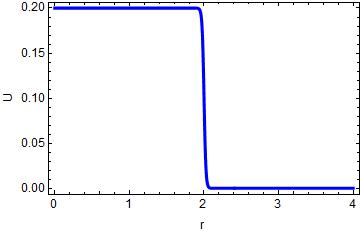
\includegraphics[width=0.9\linewidth]{PotentialTreapta}
  \caption{Poten\c{t}ial Treapt\u{a}}
  \label{fig:sub311}
\end{subfigure}%
\begin{subfigure}{.5\textwidth}
  \centering
  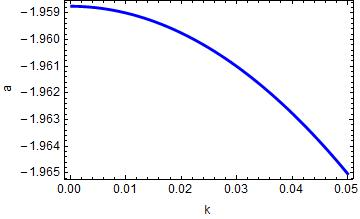
\includegraphics[width=0.9\linewidth]{LungimeImprastiereTreapta}
  \caption{Lungimea de \^{i}mpr\u{a}\c{s}tiere}
  \label{fig:sub312}
\end{subfigure}
\caption{Treapta de poten\c{t}ial}
\label{fig:treapta}
\end{figure}

\end{frame}

\begin{frame}[allowframebreaks]{Groapa de poten\c{t}ial}
\begin{align}
V({\bm r})=-V(0)\tanh{\frac{{\bm r}-r_0}{\alpha_0}}+V(0)
\end{align}
valorile parametrilor au fost p\u{a}strate
\begin{figure}[h!]
\centering
\begin{subfigure}{.5\textwidth}
  \centering
  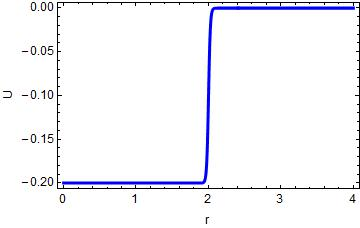
\includegraphics[width=0.9\linewidth]{PotentialGroapa}
  \caption{Poten\c{t}ial Groap\u{a}}
  \label{fig:sub321}
\end{subfigure}%
\begin{subfigure}{.5\textwidth}
  \centering
  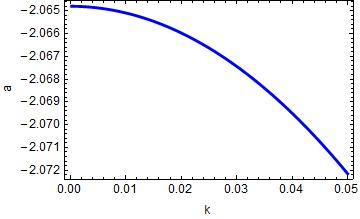
\includegraphics[width=0.9\linewidth]{LungimeImprastiereGroapa}
  \caption{Lungimea de \^{i}mpr\u{a}\c{s}tiere}
  \label{fig:sub322}
\end{subfigure}
\caption{Groapa de poten\c{t}ial}
\label{fig:groapa}
\end{figure}
\end{frame}

\begin{frame}[allowframebreaks]{Poten\c{t}ial de tip Van der Waals}
\begin{align}
V({\bm r})=V(0)\left(\left(\frac{r_0}{{\bm r}}\right)^12-2\left(\frac{r_0}{{\bm r}}\right)^6\right), \qquad \text{unde } V(0)=10^{-6}
\end{align}

\begin{figure}[h!]
\centering
\begin{subfigure}{.5\textwidth}
  \centering
  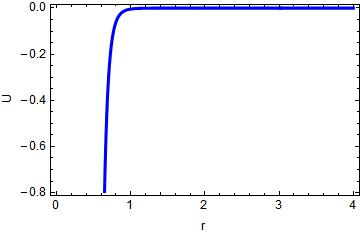
\includegraphics[width=0.9\linewidth]{PotentialVanDerWaals}
  \caption{Poten\c{t}ial de tip Van der Waals}
  \label{fig:sub331}
\end{subfigure}%
\begin{subfigure}{.5\textwidth}
  \centering
  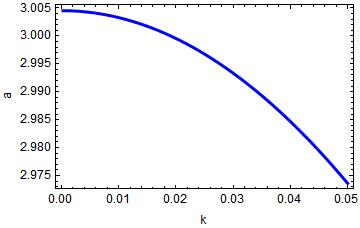
\includegraphics[width=0.9\linewidth]{LungimeImprastiereVanDerWaals}
  \caption{Lungimea de \^{i}mpr\u{a}\c{s}tiere}
  \label{fig:sub332}
\end{subfigure}
\caption{Poten\c{t}ial de tip Van der Waals}
\label{fig:groapa}
\end{figure}
\end{frame}

\subsection{Poten\c{t}ial aproximat pentru atomi de Cs}
\begin{frame}[allowframebreaks]{Poten\c{t}ial aproximat pentru atomi de Cs}
\begin{align}
V(r)=\frac{1}{2}Br^\alpha e^{-\beta r}-\left(\frac{C_6}{r^6}+\frac{C_8}{r^8}+\frac{C_{10}}{r^{10}}\right)f_c(r) \label{vcs}
\end{align}
Primul termen de dup\u{a} egal reprezint\u{a} repulsia dintre electronii de valen\c{t}\u{a}, iar al doilea reprezint\u{a} suma termenilor Van der Waals, \^{i}nmul\c{t}it\u{a} cu o func\c{t}ie de cutoff $f_c(r)$, ce are rolul de a anula divergen\c{t}a $1/r^n$ la distan\c{t}e mici.\\
Func\c{t}ia de cutoff are forma:
\begin{align}
f_c(r)=\Theta(r-r_c)+\Theta(r_c-r)e^{-(rc/r-1)^2},
\end{align}
\begin{center}
 \begin{tabular}{||c c c c c c c||} 
 \hline
 B & $\alpha$ & $\beta$ & $C_6$ & $C_8$ & $C_{10}$ & $r_c$ \\ [0.5ex] 
 \hline 
 0.0016 & 5.53 & 1.072 & 7020 & $1.1 \times 10^6$ & $1.7 \times 10^8$ & 23.165 \\ 
  \hline
\end{tabular}
\end{center}
\newpage
Prezen\c{t}a barierei \^{i}nalte \c{s}i largi face ca la energii mici propagarea solu\c{t}iei ``pe sub barier\u{a}" s\u{a} duc\u{a} la pierderea complet\u{a} a preciziei.
\begin{figure}[h!]
  \centering
  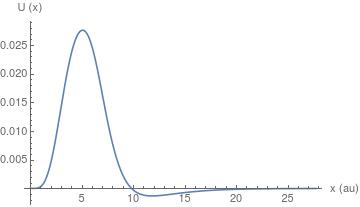
\includegraphics[scale = 0.8]{CS.jpg}
  {\caption{Potentialul (\ref{vcs})\label{gvcs}}}
  \end{figure}
  \^{I}n figur\u{a} este reprezentat\u a solu\c tia $\chi(r)$ g\u asit\u a cu Mathematica pentru $k=0.05$ u.a. Este evident c\u a solu\c tia nu are comportarea corect\u a la distan\c te mari.
\begin{figure}[h!]
  \centering
  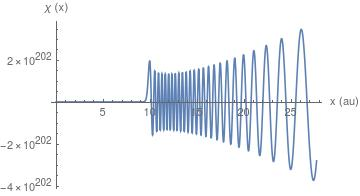
\includegraphics[scale = 0.8]{FIG.jpg}
  {\caption{Solu\c{t}ia $\chi(r)$ pentru poten\c{t}ialul (\ref{vcs})\label{figpsi}}}
  \end{figure}
  
\end{frame}

\section{Concluzii}
\begin{frame}[allowframebreaks]{Concluzii}

\begin{itemize}
\item \^{I}mpr\u{a}\c{s}tierea pe poten\c{t}iale simple, care prin rezolvarea ecua\c{t}iei Schr\"{o}dinger dau o solu\c{t}ie cu comportament agreabil, poate fi descris\u{a} \^{i}n limita de energii joase printr-un singur parametru: lungimea de \^{i}mpr\u{a}\c{s}tiere.
\item Un poten\c{t}ial mai complex, care are valori mult mai mari dec\^{a}t energia va introduce \^{i}n solu\c{t}ia ecua\c{t}iei Schr\"{o}dinger fluctua\c{t}ii prea mari pentru a mai ob\c{t}ine un rezultat corect prin metoda demonstrat\u{a}. \^{I}n acest caz sunt mai potrivite metode de evaluare a defazajului bazate pe aproxima\c tia JWKB sau pe calculul direct al fazei solu\c tiei radiale
\end{itemize}

\end{frame}

\section{Bibliografie}
\begin{frame}[allowframebreaks]{Biliografie}
\begin{thebibliography}{1000}
\bibitem{art-VW}G. F. Gribakin, V. V. Flambaum, Phys. Rev. A {\bf 48}, 546 (1993).

\bibitem{Zettili}Nouredine Zettili, Quantum Mechanics Concepts and Aplications, 2nd ed

\bibitem{varenna}Jean Dalibard, Collisional dynamics of ultra-cold atomic gases

\bibitem{Szmytk}Radoslaw Szmytkowski, Analytical calculations of scattering lenghths in atomic physics, J. Phys. A: Math. Gen. 28 (1995) 7333-7345
  
\bibitem{IHP-2007}Claude Cohen-Tannoudji. Atom-atom interactions in ultracold gases. DEA. Institut Henri Poincar\`{e}, 25 et 27 Avril 2007, 2007. $<$ cel-00346023 $>$

\bibitem{Jullienne-RMP-ColdCollisions}John Weiner, V. S. Bagnato, S. Zilio, Paul S. Jullienne, Rev. Mod. Phys, Vol 71, No. 1, January 1999

\bibitem{ris}H. Ouerdane, M. Jamieson, D. Vranceanu and M. Cavagnero, J. Phys. B  {\bf 36}, 4075 (2005).
\end{thebibliography}
\end{frame}


%%% Local Variables:
%%% mode: latex
%%% TeX-master: "../main"
%%% End:
